\chapter{NP-Completeness}

\begin{descr}
  Definition and analyisis of different complexity classes
\end{descr}

\subsection{Motivation/Examples}
\begin{tabular}{p{5cm}|p{5cm}}
  Solvable in Polinomial Time & NP complete \\
  \hline
  \deftxt{Euler Path} "a path with all edges" & \deftxt{Hamiltonian Path} "node ocurs exactly once" \\
   Shortest path from X to Y $\Rightarrow$ \deftxt{Dijkstra's}algorithm & longest simple Path between X and Y \\
  \hline
  2-CNF (conjuntive normal form) e.g. $(x_{1} \lor \lnot x_{2}) \land (\lnot x_{1} \lor x_{3})$ Can we find an assignment, that the formula becomes true in poly. time? & 3-CNF \\
  \hline
  Two processor scheduling & 3 or more processor schedulung $\Rightarrow$ NP-complete or unknown \\
  \hline
  Football game until 1955 loss 0 points, draw 1 point, win 3 points. The season has already started, is my team still able to win the championchip? & loss 0 points, draw 1 point, win 3 points \\
\end{tabular}

\subsection{Introduction}
\begin{definition}
  P is the class of problems that can be solved in polinomial time.\\

  NP is the class of porblems, where given a solution one may check in polinomial time, that it is indeed one.
\end{definition}

\begin{example}
Example:
\begin{enumerate}
  \item Given a connected undirected-finite graph. Is there a circle such taht every node appears exatly once on the circle.
        Given such a circle $< v_{1},...v_{n}>$ it can easily checked that it has the property. $\Rightarrow$ Hamiltonian Cycle $\in$ 
        NP.
  \item 3-CNF; given values for the variables, we can check that the formula becomes true, with this values in polynomial time.
\end{enumerate}

\textbf{Clarity:} $P \subseteq NP$ open problem; $P = NP ??$

Overview: \\
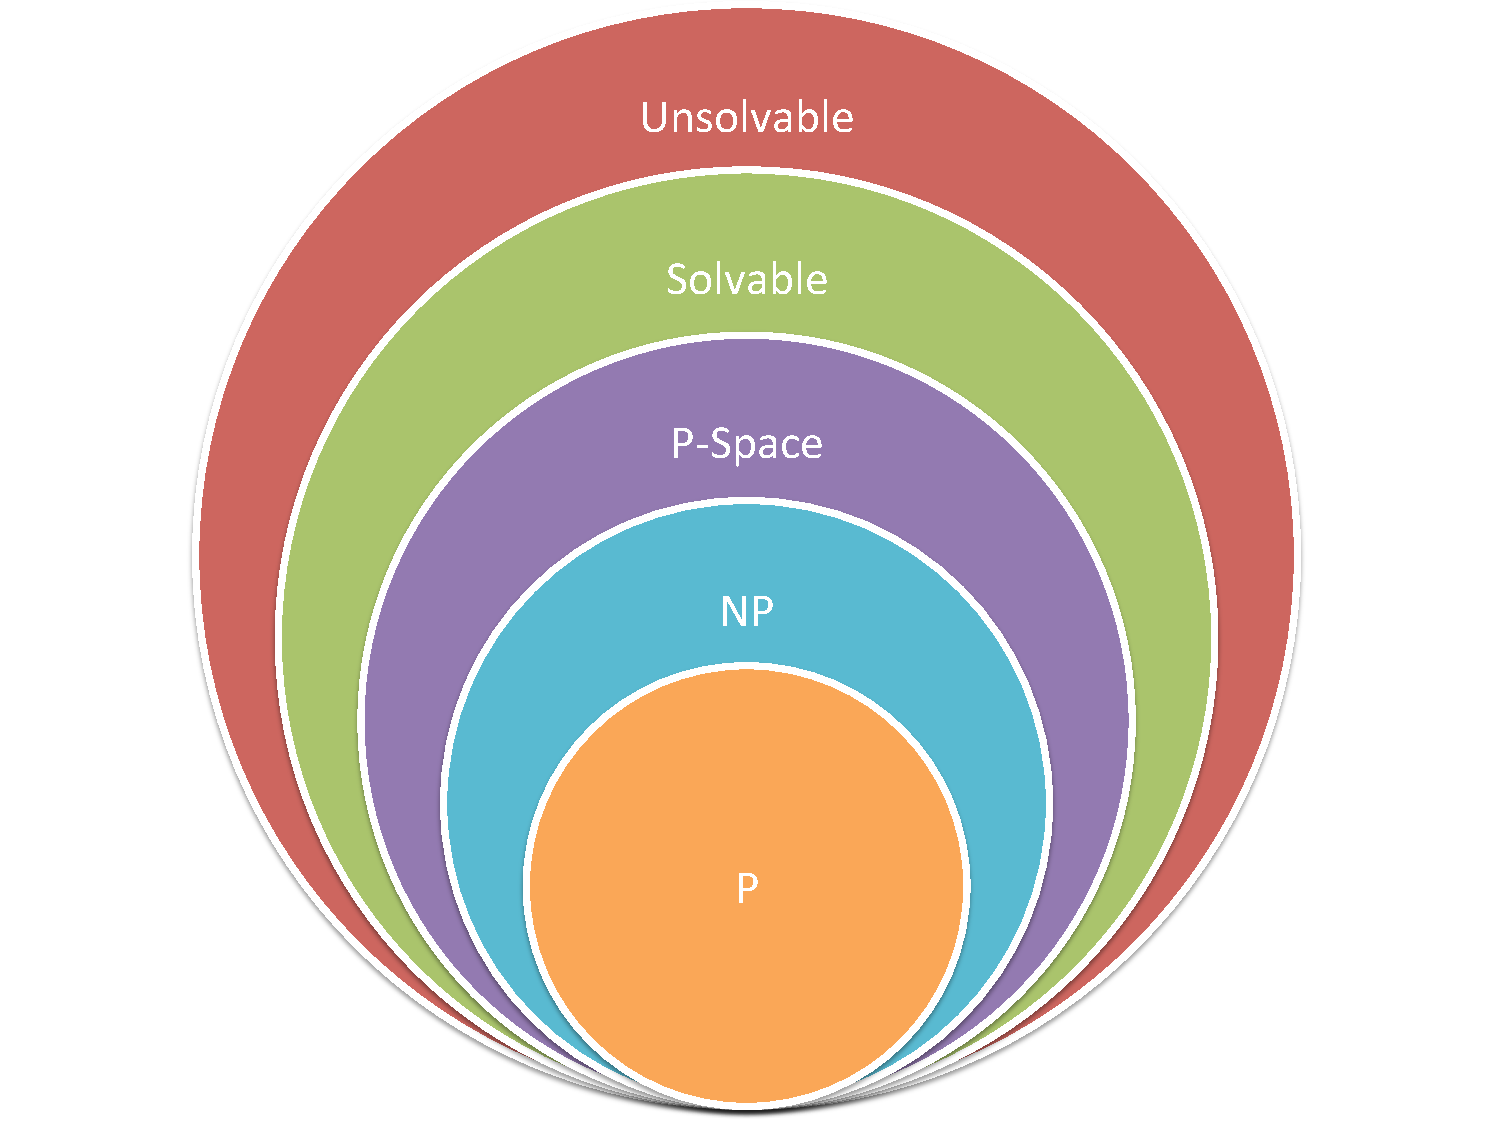
\includegraphics[scale=0.3]{diagrams/comp_classes}
\end{example}

\subsection{Problem Types/Issues}

\begin{tabular}{p{5cm}|p{5cm}}
  \textbf{Decision Problems} & \textbf{Optimization Problems} \\
  \hline
  Yes or no answer, is there a path from X to Y? & Find the shortest path from X to Y?
\end{tabular}

\begin{definition}
  Complexity Theory deals with \deftxt{decision problems}. Optimization problems are tried to transform into decision problems.
\end{definition}

\begin{example}
  Choose an integer k, treat the decision problem: "Is there a path from X to Y no longer than k?"
\end{example}  

To show that an optimization problem is hard to solve it is sufficient to consider the related decision problem. If the latter is hard to solve, so is the first. \\

\textbf{Reductions} \\
Reductions are used to show that problem are hard to solve. A reduction reduces a decision problem to another one.\\
$A \Rightarrow B$ (reduction)

Properties of the reduction should be: "it can be done in polynomial time". \\
If $A$ and $B$ the transformation of $A B$ is an instance of $B$ then $A$ should have the answer yes if and only if $\beta$ has the answer yes.\\
Call this a \deftxt{polynomial reduction}.\\
If $A \rightarrow B$ and $B$ can be solved in poly. time, then instances of $A$ can be solved in poly. time. \\
If $A \rightarrow B$ and $A$ is hard to solve, then we may conclude that  $B$ is hard to solve. \\
\newline
Lecture of 08.05.13 - beginning: redundancy to former parts? \\
\\ Consider the following classes: P, NP, NPC \\
Class $A \xrightarrow{poly} B$ \\
Instance $\alpha \rightarrow \beta$ \\

\begin{enumerate}[label={\arabic* Observation:}]
  \item If the instances of the problem B can be solved in poly time, then this is true for instances of A.
  \item If the instances of A are "hard" to solve, so are the instances of B.
  \item If A is in NPC and $B \in NP$, then we can conclude B is also in NPC.
\end{enumerate}
Problem: To find a first problem class in NPC (St. Cook 1971 3-SAT problem)

\section{Polynomial Time}

\begin{enumerate}[label={\arabic*.}]
 \item Problem solvable in $O(n^100)$? \\
       Speed-up theorem of Blum $\rightarrow$ reduce export
 \item Polynomial time is independent of the computer model
 \item The class of polynomials is closed with respect to addition, multiplication and compostion.
 \item Practical reasons.
\end{enumerate}
 
\begin{definition}[Abstract Decision Problem]
  An \deftxt{Abstract Decision Problem} is a mapping $\mathbb{Q}:I \rightarrow \{0,1\}$.
  $I$: is a set of problem instances
\end{definition}

\begin{example}
  Is there a path from u to v in the directed graph G of length $\leq$ k $I=\{ (G,u,v,k): k \in \mathbb{N}, G \text{ finite directed Graph, u,v are nodes in G }  \}$ \\
  $Q( (G,u,v,k) ) = 1$ if $\exists$ path ... and $Q( (G,u,v,k) ) = 0$ otherwise.
\end{example}

\subsection{Conding and concrete problems}

A \underline{coding} of as set S is a mapping $e: S \rightarrow \{0,1\}$. \\
A concrete problem is a problem, the instances of which are in \{ 0,1 \}. \\
$Q: S' \leq \{ 0,1 \} \rightarrow \{ 0,1 \}$ \\
An algorithm solves a concrete problem in $O(T(n))$ if it delivers the answer for an input x with $\left| x \right| = n$ on $O(T(n))$ steps. \\
A concrete problem is said to be solvable in polynomial time if there is an algorithm solving it in $O(n^k)$ for some k.\\
P is the class of concrete problems that can be solved in poly time. \\
Let $Q:I \rightarrow \{ 0,1 \}$ be an abstract problem and $e:I \rightarrow \{ 0,1 \}^*$ be an encoding.\\
The resulting concrete problem $Qe: e(I) \rightarrow \{ 0,1 \}$ such that $Q(i) = 1$ iff $Qe(e(i)) = 1 \subseteq
 \{ 0,1 \}^*$.
 
\begin{example}
  Consider an algorithm for an abstract problem an $\mathbb{N}$ that needs $\Theta(k)$ steps for input $k \in \mathbb{N}$. \\
  \underline{encoding e:} $\mathbb{N} \rightarrow \{ 0,1 \}$ $e(k) = 11111$ (k times), then the algorithm is linear in the length of the input. \\
  \underline{encoding e':} $e'(k)=$binary representation of k length$e'(k) = \left| e'(k) \right| = \log_2 k +1$ (log hat eigentlich so eckige klammern)
\end{example}

The algorithm with this encoding produces costs exponential in the length $\left| e'(k) \right|$ of the input $f:\{ 0,1 \}* \rightarrow \{ 0,1 \}*$ is said to be compatible in poly time if there is an algorithm that computes $f(x), x \in \{ 0,1 \}*$ in poly time.

Two encodings are called polinomically connected if there are two functions $f_{12}$ and $f_{21}$ with $f_{12}(e_{1}(i)) = e_{2}(i), f_{21}(e_{2}(i)) = e_{1}(i), i \in I$ that are polinomially computable.\\

\begin{samepage}
\begin{lemma}
  Let $Q$ be an abstract decision problem. \\
  $Q:I \rightarrow \{ 0,1 \}$ \\
  $e_{1},e_{2}:I \rightarrow \{ 0,1 \}*$ encodings that are polynomially connected, then $Q_{e_{1}} \in P$ iff $Q_{e_{2}} \in P$
\end{lemma}
\end{samepage}

\begin{proof}
  Steps:
  \begin{enumerate}
    \item $Q_{e_{1}}: e_{1}(I) \subseteq \{ 0,1 \}* \rightarrow \{ 0,1 \}$ be solvable in $O(n^k)$ for some k for input of length n
    \item Let $e_{1}(i)$ be computable from $e_{2}(i)$ in $O(n^c)$ where $n=\left| e_{2}(i) \right|$. \\
          We want to show, that $Q_{e_{2}} \in P$ to solve $Q_{e_{2}}$ we proceed as follows: \\
          $Q_{e_{2}}: e_{2}(I) \rightarrow \{ 0,1 \}$ consider $e_{2}(i)$. First determine $e_{1}(i)$ from $e_{2}(i)$ and then run the algorithm for $Q_{e_{1}}$ on the input $e_{1}(i)$.\\
          The first step costs $O(n^c), n= \left| e_{2}(i) \right|$ and the result is $e_{1}(i)$.\\
          In th second step the algorithm for $Q_{e_{1}}$ is run on $e_{1}(i), \left| e_{1}(i) \right| = O( \left| e_{2}(i) \right|^c)$. \\
          It needs $O((n^c)^k) = O(n^{ck})$ \\
          \newline
          Sidenote: length $\rightarrow \left| e_{1}(i) \right| \leq O(n^2) \rightarrow P \leq PSPACE$
  \end{enumerate}
\end{proof}

\section{Formal Language Representation}
Let $\epsilon$ be an alphabet (=finite set, the elements are called symbols).\\
A language over $\epsilon$ is a subset of $\epsilon^*$, $\epsilon^*$ all finite sequences of over $\epsilon$.\\
$L \leq \epsilon^*$ (Grammar density?)\\
\newline
Start lecture on 13.05.2013\\
\newline
\textbf{Decidability vs. Acceptance}\\
$\epsilon$ finite set of symbols, $\epsilon^*$ all finite sequences.\\
Language is $L \subseteq \epsilon^*$. \\
Let $Q$ be a concrete decision problem $L = \{ x \in \{ 0,1 \} \} Q(x) = g??$. An algorithm A accepts its output\\
\textbf{Sentence Missing!!} \\
A \deftxt{rejects} x if $A(x) = 0$.

A \deftxt{decides} a language $L = \{ x \in \{ 0,1 \}^* \}$ if $A(x) = 1 \forall x \in L$ and $A(x) = 0 \forall x \not\in L$. L is accepted by A in polynomial time, if A accepts L and there is a $k \in \mathbb{N}$, such that for every $x \in L$, if $\left| x \right| = n$ A accepts x $O(n^k)$ with $n \in \mathbb{N}$. 

Algorithm A decides L in polynomial time if there is $k \in \mathbb{N}$ such that if $\left| x \right| = n$ then A decides if $x \in L$ in $O(n^k)$.

Given a programm $P_{r}$ and input y, the question: "Will P terminate?" is \deftxt{undecidable}" \textbf{!important theorem!}.\\
But there is an algorithm $\{(P_{r},y):P_{r} ~ \text{terminates on y} \}$ that can be accepted. \\
Now we can defer the class $P=\{ L \subseteq \{ 0,1 \}^*: \exists ~\text{algorithm deciding L in polynomial time} \}$.

\begin{lemma}
  $P=\{ L \subseteq \{ 0,1 \}^*: \exists ~\text{algorithm that accepts L in polynomial time} \}$.
\end{lemma}

\begin{proof}
  Each problem that can be decided (in polynomial time) can be accepted (in polynomial time). Let L be accepted in polynomial time
  by an algorithm A, that there is a $k \in \mathbb{N}$ such that for each $\left| x \right| = n$ A accepts $x \in L$ in $O(n^k)$.\\
  So an algorithm deciding L, works as follows:\\
  Let $x \in \{ 0,1 \}$ with $\left| x \right| = n$ be given. Run algorithm A $O(n^k)$ steps. If it delivers 1 then deliver 1,
  otherwise 0, beacuse if x was in L, the answer 1 must have been produced with $O(n^k)$ steps.
\end{proof}


\section{Polynomial Verification}
A verification algoritm is an algorithm with two input parameters $A(x,y)$. \\
A verifies x if there is a y with $A(x,y) = 1$.\\
Y is called a certificate.\\
$L=\{ x \in \{ 0,1 \}^*: \exists ~ y \in \{ 0,1 \}^*:~A(x,y)=1\}$ the langugage verified by A.\\

A language belongs to the class NP if there is a polynomial time verification algorithm A and a constant c such that: \\
$L=\{ \underbrace{x \in \{ 0,1 \}^*}_{\text{a graph}}: \underbrace{\exists y}_{\text{Hamiltonian Cycle}} ~\text{with}~ \left|y \right|=O(\left| x \right|^c) ~\text{and}~ \underbrace{A(x,y)=1}_{\text{algo that shows that y is a Hamiltonian Cycle}}\}$  \\
We say A verifies L in polynomial time.\\
\vspace{0.3cm}
Some complexity classes and their relationships:\\
$\text{co-NP} = \{ L: \epsilon^* \backslash L \in NP  \}$\\
$\text{co-AnyClass} = \{ L: \epsilon^* \backslash L \in \text{AnyClass} \}$
So far proofen or not:\\
$P \subseteq NP$ \\
$P \stackrel{?}{=} NP$ \\
$P \stackrel{?}{=} \text{co-NP} \cap \text{NP}$ \\
$\text{co-NP} \stackrel{?}{=} NP$ \\

\section{NP-completeness and reducability}
$L_{1}$ is reducable in polynomial time to $L_{2}$ ($L_{1} \leq_{p} L_{2}$) if there is a function f computable in poly. time
with: \\
$x \in L ~\text{iff}~ f(x) \in L_{2} ~f:\{ 0,1 \}* \rightarrow \{ 0,1 \}*$\\
f is called a reduction function\\
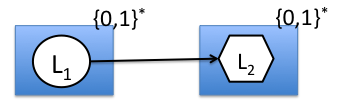
\includegraphics[scale=0.5]{diagrams/reductions}

\begin{lemma}
  $L_{1}, L_{2} \in \{ 0,1 \}^*$ and $L_{1} \leq_{p} L_{2}$.\\
  If $L_{2} \in P$ then $L_{1} \in P$.
  \vspace{0.3cm}
  $L \in \{ 0,1 \}^*$ is called \deftxt{NP-complete} (NPC) if
  \begin{enumerate}
    \item $L \in NP$
    \item $L' \leq_{p} L \forall L' \in NP$
  \end{enumerate}
  If L satisfies ii) L is called \deftxt{NP-hard}.\\
  $\text{NPC} = \{ L: ~ \text{L is NP-complete} \}$
\end{lemma}

\begin{lemma}
  If some L in NPC can be solved in polynomial time, then $P=NP$.\\
  If there is a $L \in NP$ that cannot be solved in poly. time then no problem in NPC can be solved in polynomial time.
\end{lemma}

\begin{lemma}
  If $L' \in \text{NPC}$ and $L' \leq_{p} L$ the $L$ is NP-hard.
\end{lemma}

\begin{proof}{}
 $L' \in NPC$ and $\forall L'' \in NP$ it holds $L'' \leq_{p} L'$ $L' \leq_{p} L$ \\
 $">"$ $\forall L'' \in \text{NP}$ $L'' \leq_{p} L$
\end{proof}

\vspace{0.3cm}
The first problem to show NP-complete (remember check for NP $\rightarrow$ check in poly. time if you have a solution): \deftxt{SAT}. Satisfiablility of Boolean Formulas (Cook 1971)\\
The second problem to show NP-complete: 3-SAT. $\text{SAT} \leq_{p} \text{3-SAT}$